%%%%%%%%%%%%%%%%%%%%%%%%%%%%%%%%%%%%%%%%%%%%%%%%%%%%%%%%%%%%%%%%%%%%%%%%%%%%%%%%%%%%%%%%%%%%%%%%%%%%%%%%%%%%%
%
% witseiepaper-2005.tex
%
%                       Ken Nixon (12 October 2005)
%
%                       Sample Paper for ELEN417/455 2005
%
%%%%%%%%%%%%%%%%%%%%%%%%%%%%%%%%%%%%%%%%%%%%%%%%%%%%%%%%%%%%%%%%%%%%%%%%%%%%%%%%%%%%%%%%%%%%%%%%%%%%%%%%%%%%%

\documentclass[10pt,twocolumn]{article}

%
% All KJN's macros and goodies (some shameless borrowing from SPL)
\usepackage{KJN}
%\usepackage{a4wide}
\usepackage{fullpage}
\usepackage{textcomp}
\usepackage{url}
\usepackage{fancyvrb}
\usepackage{amsfonts}
\usepackage{amsmath}
\usepackage{algorithm}
\usepackage{titlesec}
\usepackage{enumitem}
\usepackage{subcaption}

\setcounter{secnumdepth}{5}

\newcommand{\K}{\textit{k }}
\newcommand{\M}{\textit{m }}
\newcommand{\N}{\textit{n }}
\newcommand{\D}{\textit{d}}
\newcommand{\PP}{\textit{p}}
\newcommand{\QQ}{\textit{q}}

%%%%%%%%%%%%%%%%%%%%%%%%%%%%%%%%%%%%%%%%%%%%% PDF Info %%%%%%%%%%%%%%%%%%%%%%%%%%%%%%%%%%%%%%%%%%%%%%%%%%%%%%

\ifpdf
\pdfinfo{
/Title (Parallel  Haplotyping Assembly : Xeon Phi vs. Nvidia K20x )
/Author (Robert Clucas)
/CreationDate (D:200309251200)
/ModDate (D:200510121530)
/Subject (ELEN4002 Laboratory Project, 2015)
/Keywords (Haplotyping, GPU, Branch, Bound, Simplex)
}
\fi

%%%%%%%%%%%%%%%%%%%%%%%%%%%%%%%%%%%%%%%%%%%%%% TITLE ETC %%%%%%%%%%%%%%%%%%%%%%%%%%%%%%%%%%%%%%%%%%%%%%%%%%%%

\begin{document}

\title{Parallelizing the Haplotying Assembly Problem}

\author{Robert Clucas - 541590}

%%%%%%%%%%%%%%%%%%%%%%%%%%%%%%%%%%%%%%%%%%%%%%% ABSTRACT %%%%%%%%%%%%%%%%%%%%%%%%%%%%%%%%%%%%%%%%%%%%%%%%%%%%

%\keywords{Brach, Bound, GPU, Haplotyping, Simplex}

\maketitle
\pagestyle{plain}

\abstract{This report details the haplotype assembly problem, specifically the minimum error correction
    formulation. An algorithm for solving the minimum error correction formulation of the problem is chosen
    for parallelization which is based on integer linear programming and is known to be NP hard. The branch
    and bound algorithm is chosen as the method for solving the problem. Possible parallel implementations 
    of both the pre-processing of the input data and the branch and bound algorithm are provided, which aim to
    reduce the long run times required by current implementations to solve the problem. The project will be
    implemented using multi-core CPUs, Intel Xeon Phi coprocessors, and Nvidia GPUs. The software will be
    written using C and C++, and only free software will be used. The CUDA and OpenMP libraries will be used
    for the Nvidia GPUs and for communication between CPU threads, respectively.
}

%%%%%%%%%%%%%%%%%%%%%%%%%%%%%%%%%%%%%%%%%%%%%%%% BODY %%%%%%%%%%%%%%%%%%%%%%%%%%%%%%%%%%%%%%%%%%%%%%%%%%%%%%%

\pagestyle{plain}

\section{Introduction}

It is commonly accepted that all humans share $\mathtt{\sim}$99$\%$ of the same DNA, however, small variations 
cause human beings to have different physical traits. Single nucleotide polymorphisms (SNPs), which are
variations of a single DNA base from one individual to another, are believed to be able to address
genetic differences. For diploid organisms, which have pairs of chromosomes, a \textit{haplotype} is a 
sequence of SNPs in each copy of a pair of chromosomes. A \textit{genotype} describes the conflated data of the
haplotypes on a pair of chromosomes. Haplotypes are believed to contain more generic information than
genotypes \cite{stephens:2001}, however, obtaining haplotypes correctly is a difficult problem, which has been
studied in two main forms : haplotype inference and haplotype assembly (HA). 

Haplotype inference uses the genotype of a set of individuals. The genotype data tells the status of each
allele at a position, but does not distinguish which copy of the chromosome the allele came from.
The negative aspects of this approach are that it cannot distinguish rare and novel SNPs \cite{he:2010}, 
and there is no way of knowing if the inferred haplotype is completely correct. 

Haplotype assembly uses fragments of sequences generated by sequencing technology to determine
haplotypes. The fragments of a sequence come from the two copies of an individual's chromosome. The goal of the
haplotype assembly problem is then to correctly determine two haplotypes, where each haplotype corresponds to
one of the two copies of the chromosome. Table~\ref{tab:exinp} in Appendix~\ref{app:inpre} shows an example
input, where $h$ and $h'$ are the assembled haplotypes. 

The haplotype assembly problem was proven to be NP hard \cite{lippert:2002}. The algorithms used to solve the
problem are thus computationally expensive and until recently, there was no practical exact algorithm to solve 
the minimum error correction (MEC) formulation of the problem \cite{bonizzoni:2003},
However, recently an exact algorithm was proposed by \cite{chen:2013} which is capable of solving the MEC 
formulation exactly, and can thus correctly infer all haplotypes from the fragment sequences. Due the problem
being NP hard, the implementation requires a long time to solve the problem - in the range of days for chromosomes with high
errors rates. A parallel implementation could reduce the long run time, 
allowing useful haplotype information to be more quickly inferred from the available datasets, having
positive effects in fields such as drug discovery, prediction of diseases, and variations in gene
expressions, to name a few. 

Parallel programming makes use of devices which have numerous cores, and uses these cores to execute a single
instruction on multiple data (SIMD). The effectiveness of parallel programming is dependant on the nature of 
the problem, as per Amdahl's law. While using multiple processors can potentially provide large performance 
increases, in practise the performance improvements are difficult to achieve due to additional complexities 
which are introduced by parallelism. The main difficulties are the synchronization and communication between 
the multiple cores, and the management of memory between the host (normally a CPU) and the device (parallel
capable hardware, a GPU for example). Threads are created to operate on some data in parallel, and a block of
threads is allocated memory which is accessible only to the threads in the block, while all threads from all
blocks have access  to a global memory space, however, access to this  memory space is slower, decreasing 
performance. Furthermore, race conditions, where multiple threads attempt to access data at the same location 
simultaneously, can cause undefined behaviour and hence inaccurate results.

With the increasing popularity of General-Purpose GPU (GPGPU) programming, however, API's like CUDA
\cite{nvidia:2015} and OpenCL \cite{khronos:2015}
which provide access to GPUs through simple function calls in C and C++, have made parallel programming
easier on GPUs. Intel have also started to provide parallel focussed hardware, introducing the Xeon Phi, which, like 
a GPU, has numerous cores which can operate on data in parallel. The Xeon Phi is also programmed using an API 
\cite{intel:2013}, however, far more extensive use is made of compiler directives than by CUDA or OpenCL, 
with API functions being provided to gain access to parallel variables such as the thread index and number of 
threads which are running in parallel. Using these APIs, it is possible to write parallel implementations of
algorithms which have significantly shortened run times.

The contribution of this paper is to consider the proposed algorithms for solving the HA problem, then to
choose one for which parallelization can potentially provide performance improvements, and then to identify 
components of the selected algorithm which would be suited for parallelism, as well as proposing possible 
parallel implementation of the identified parallelizable components. Additionally, this paper details the
specifications of the project and breakdown of work such that the project will be completed by the deadline.

The remainder of this paper is structured as follows. Section~\ref{sec:bground} provides background
information related to the HA problem, some of the proposed algorithms for solving it, the MEC
formulation, and the branch and bound algorithm. Section~\ref{sec:projdes} describes the specifics of the
project. Section~\ref{sec:proc} presents the general procedure for solving the chosen algorithm. 
Section~\ref{sec:parpre} describes possible parallelization of the pre-processing of the input data. 
Section~\ref{sec:parbnb} describes the parallelization of the branch and bound algorithm, which is the chosen
algorithm for solving the problem. Section~\ref{sec:conc} concludes.

%%%%%%%%%%%%%%%%%%%%%%%%%%%%%%%%%%%%%%%%%%%%%%%%%%%%%%%%%%%%%%%%%%%%%%%%%%%%%%%%%%%%%%%%%%%%%%%%%%%%%%%%%%%%%

\section{Background} \label{sec:bground}

\subsection{Haplotype Asembly Problem} \label{sec:hap}

This subsection will provide a brief overview of the haplotype assembly problem, and define the
notation used through the rest of the paper. The input to the problem is a set of reads from a given genome
sequence, where each read contains fragments from each of the two chromosomes which make up the genome
sequence. The characters of a read consist of elements from a \textit{ternary string}, where a ternary
string has characters from the set \{0, 1, -\}. A value of 0 refers to the major allele
at a site, a value of 1 to the minor allele, and a value of - to the lack of a read at the site, and is
referred to as a \textit{gap}. These reads are then combined to form a matrix, where each row of the 
matrix corresponds to a read (Table~\ref{tab:exinp} in Appendix~\ref{app:inpre} provides an example). 

Each column of the matrix is known as an SNP site. At each site, the data could be accurate, missing, or have
error. The goal of the haplotype assembly problem is to determine a haplotype, H = \{\textit{h,h'}\}
from the matrix. The following terminology will be used to refer to properties of the input matrix and the
fragments. 

For the input matrix, M, the number of fragments is denoted by \textit{m}, which is the number of rows in M.
The number of SNP sites is denoted by \textit{n}, which is the number of columns in M, while the j$^{th}$ 
site of the i$^{th}$ fragment is given by \textit{f$_{ij}$}. Two fragments are said to 
conflict if the following conditions are true:
\begin{itemize}
    \item{f$_{ik}$ $\neq$ f$_{jk}$ \textbf{and} f$_{ik}$ $\neq$ `-' \textbf{and} f$_{jk}$ $\neq$ `-' }
\end{itemize}
Essentially this means that for two fragments i and j, if at an SNP site k, the reads do not have error and are 
not gaps, the reads have different values (fragment i has a value 0 at site k, while fragment j has a value 
1 at site k, or vice versa). 

Following the notation of a conflict, the \textit{distance} between two fragments is
denoted by d(f$_i$, f$_j$), and is the total number of positions for which the two fragments f$_i$ and f$_j$
conflict. Furthermore, to understand some of the problem formulations from the fragment data, it is useful to
define a \textit{conflict graph} G = \{V, E\} \cite{lancia:2001}, where V corresponds to a fragment, and E
corresponds to an edge between two fragments if they conflict. If the input matrix contains no errors, then none
of the fragments from the same chromosome will conflict and G will be bipartate. However, if there are 
errors (as is often the case) in M, G will not be bipartate. The haplotype assembly problem then requires 
the correction of G from a non-bipartate graph to a bipartate graph, from which two haplotypes can be
assembled. There are numerous methods for solving the problem:
\begin{itemize}[noitemsep]
    \item{ \textbf{Minimum Fragment Removal (MFR):} This invloves removing the least number of fragments 
            from the input data such that the resultant graph G is bipartate. It is shown in 
            \cite{lancia:2001} that this can be solved in polynomial time.
        }
\item{ \textbf{Minimum Edge Removal (MER) \cite{aguiar:2012}:} This method was recently proposed, and requires
        determining the minimum number of edges to remove such that removal of the edges results in G being 
        bipartate.
    }
\item{ \textbf{Longest Haplotype Reconstruction (LHR):} This requires finding a set of fragments which,
        when they are removed from M, result in G being bipartate and the length of the resultant 
        haplotypes being maximized \cite{schwartz:2010}. 
    }
\item{ \textbf{Minimum Error Correction (MEC):} This method involves correcting the minimum number of 
        elements (sites for all fragments) in M which allows the graph G to be bipartate. 
        Although being the most complex method, it is the most widely used method as it provides the 
        highest accuracy. Only recently has an exact algorithm for the MEC formulation been proposed which 
        can provide an exact solution for all cases.
    }
\end{itemize}
Due to the accuracy and more extensive previous work, the MEC formulation of the HA problem was chosen for a
parallel implementation, hence will be the focus for the remainder of the paper.

\subsection{Minimum Error Correction Formulations} \label{sec:mecimp}

Much research has been done on solving the MEC formulation of the HA problem. The first exact algorithm for
solving the problem was a branch and bound algorithm proposed by \cite{wang:2005}. The algorithm creates a
tree which covers the search space of all possible corrections. The tree is then traversed to find the best
solution. They use an upper bound which allows branches to be pruned when a better solution than the current 
best cannot result from further exploration of the branch, resulting in faster run times. However, this exact 
method has time complexity of O(2$^{\textit{m}}$), where \M is the number of fragments in the input data, and 
hence cannot determine solutions for large problem sizes within a feasible amount of time. They also 
provide a heuristic method which uses a genetic algorithm to improve the computational time, with
run times up to three orders of magnitude faster than the branch and bound implementation. While the heuristic
method gives very similar results to the branch and bound implementation, it is slightly less accurate. 

A dynamic programming solution was proposed by \cite{xie:2008} which improved the run time problem for large
input sizes. The algorithm has time complexity of O(\textit{mk}3$^{\textit{k}}$ + \textit{mlogm} +
\textit{mk}), where \K is the maximum number of SNP sites a fragment covers. In practice \K is usually small,
and results were shown small \K (less than 100). The proposed dynamic programming solution had significant run
time improvements over the solution proposed by \cite{wang:2005}. However, for larger \K values, the 
algorithm cannot solve the MEC formulation of the HA problem within a feasible amount of time. 

More recently, \cite{chen:2013} proposed an exact algorithm for solving the MEC problem. The proposed
algorithm is the currently the only algorithm which can solve the HA problem for both the \textit{all heterozygous}
case (the alleles at an SNP site are assumed to be different) and the \textit{general} case (the 
alleles at an SNP site may be the same due to error). Most other work assumes that the input fragment data is 
heterozygous, which, while true for most of the SNP sites in the input matrix, is often false for a small 
number of the SNP sites, which is the benefit of the algorithm proposed by \cite{chen:2013}. Their exact
algorithm removes unnecessary data from the input matrix, and partitions the matrix into smaller sub-matrices
(or unsplittable blocks to use their terminology, Appendix~\ref{app:inpre} provides an example) which can then 
be solved in parallel. The problem is then formulated as an \textit{integer linear programming} (ILP) problem 
and solved as a minimization problem. Their implementation was tested using an Intel i7-3960X CPU. For the 
HuRef dataset, the implementation required 12 days to solve the general case, and 31 hours for the all heterozygous case. 
Heuristics methods are also proposed which speed up the computation by up to 15 times. However, the results 
are only shown for smaller input sizes, and the heuristic methods does  not always determine the optimal 
solution. Most importantly, the solutions for the general case show lower MEC scores, meaning that the 
all heterozygous assumption is not always valid. This algorithm for the MEC formulation was chosen as it
achieved optimal solutions for the all heterozygous and general cases. Their exact formulation of the problem
as an ILP problem for the al lheterozygous case is now given.

\subsubsection{All Heterozygous Algorithm by Chen} \label{sec:allhetro}

This subsection will summarize the all heterozygous ILP formulation of MEC HA problem as it is the algoirhm
which was chosen for parallelization, and is referred to throughout the remainder of the paper.

The Hamming distance between two fragments $i$ and $j$, d = ($f_i$,$f_j$), is used by \cite{chen:2013} to 
determine the MEC score of a solution H = \{$h$,$h'$\}, and is number of SNP sites at which the fragments 
conflict. Using the Hamming distance between all the fragments and the solution, the MEC score is given by
\begin{equation}
\textrm{MEC score} = \sum_{i = 1}^{m}{ min\{\D(f_i, h), \D(f_i, h')\} }
\end{equation}
Where \M is again the number of rows in the input matrix M. The MEC score is \textit{optimal} if it is the
minimum possible score. Some assumptions are made for the input matrix as per \cite{chen:2013}, namely
\begin{itemize}[noitemsep]
\item{ No row of the input matrix is useless - at least one entry in the row is a 1 or 0 
}
\item{ No column of the input matrix is monotone - the column must have at least one 0 and one 1
}
\item{ No column of M contains more 1's than 0's - if this is not the case the values are all flipped, which
    does not change the solution or the MEC score
}
\end{itemize}
The input matrix first undergoes pre-processing to reduce the size of the input and to break the input into
multiple blocks which can be solved in parallel. It must be noted that the pre-processing does not affect 
the solution in any way. The pre-processing functions which are applied are:
\begin{itemize}[noitemsep]
\item{ \textbf{Block decomposition:} This process takes the input matrix and splits it into smaller,
        unsplittable blocks, which are disjoint and can be solved independently.
}
\item{ \textbf{Singleton removal:} A singleton is a row for which the start and end positions of the fragment
    are the same - i,e the fragment has only one element. Since singletons do not affect the MEC score,
    they can be removed. This is done for all rows in all the smaller, unsplittable blocks.
}
\item{ \textbf{Duplicate removal:} Rows and columns which are the same are merged into a single row or column, 
        and the multiplicity of the row or column is recorded. This is done for all rows and all columns in
        all the smaller, unsplittable blocks.
}
\end{itemize}
Additionally for the general case, the intrinsically heterozygous columns need to be determined. 
Determining if a column $j$ is intrinsically heterozygous requires counting the number of rows in the input matrix which
have a value of 0 (1) at position $j$, which is stored as a variable $n_{j,0}$ ($n_{j,1}$), as well as the
number of non-singular rows in the input matrix which have a value of 0 (1) at position $j$, which is stored
as a variable $s_{j,0}$ ($s_{j,1}$). Column $j$ is then intrinsically heterozygous if
\begin{equation*}
    min\{n_{j,0},n_{j,1}\} \ge \left[ \frac{s_{j,0} + s_{j,1}}{2} \right]
\end{equation*}
From the reduced blocks the ILP problem is formulated for the all heterozygous and the general case. The
all heterozygous case formulation will be shown, the general case formulation is shown in \cite{sup:2013}. 

\paragraph{ILP Formulation} \label{ssec:ilpform}

For integers \PP,\ \QQ\ $\in$ $\mathbb{Z}$, where 1 $\le$ \PP\ $\le$ \M, and 1 $\le$ \QQ\ $\le$ \N, \PP\ is the 
index of the fragment (or row) in the input matrix, M, and \QQ\ is the index of SNP (or column) in M. 
The multiplicity of the $j^{th}$ column of M is denoted by $c_j$, while the multiplicity of the
$i^{th}$ row of M is denoted by $c_j$. The following 
binary variables are introduced, $y_i$, which has a value of 1 if \D($f_i$, h) $\le$ \D($f_i$, h'), otherwise 
has a value of 0 (when \D($f_i$, h') $<$ \D($f_i$, h)). Informally, if fragment $i$ is part of $h$ then $y_i$ 
has a value of 1, otherwise it has a value of 0. $x_j$, which has a value of 1 if the $j^{th}$ bit of 
$h$ is 1, otherwise has a value of 0 (if the $j^{th}$ bit of $h$ is 0). 
Lastly $J_{i,0}$ ($J_{i,1}$) are the sets of integers $j \in \{1,2,...,q\}$ for which 
the $i^{th}$ value in column $j$ is a 0 (1). An example of the ILP formulation is is given in 
Appendix~\ref{app:ilpex}.

Using the above defined variables, an integer programming formulation is possible, however, a non-linear 
term in the form of $y_ix_j$ arises, which cannot be solved using ILP techniques. To overcome this problem, 
\cite{chen:2013} defines a variable $t_{i,j}$ for $y_ix_j$ and imposes constraints on the variable which 
ensure linearity (the constraints are shown in the final formulation of the problem below). The final ILP 
formulation of the HA problem for the all heterozygous case is 
\begin{equation*}
\begin{split}
    \textrm{Minimize} 
    &\ \ \ \sum_{i = 1}^{p}{w_i} \sum_{j \in J_{i, 0} }^{}{c_j(1 - x_j - y_i + 2t_{i,j})}                 \\
    &+ \sum_{i = 1}^{p}{w_i} \sum_{j \in J_{i, 1}}^{}{c_j(y_i + x_j - 2t_{i,j})}                
\end{split}
\end{equation*}
\begin{equation*}
\begin{split}
    \textrm{Subject to} 
    &\ \ \ \ \forall_{1 \le i \le p} \ \ y_i \in \{0, 1\}                                                 \\
    &\ \ \ \ \forall_{1 \le j \le q} \ \ x_j \in \{0, 1\}                                                 \\
    &\ \ \ \ \forall_{1 \le i \le p} \ \ \forall_{1 \le j \le p} \ \ t_{i,j} \in \{0, 1\}                 \\
    &\ \ \ \ \ \ \ \ \ \ \ \ \ \ \ \ \ \ \ \ \ \ \ \ \ \ t_{i,j} \le y_i                                  \\ 
    &\ \ \ \ \ \ \ \ \ \ \ \ \ \ \ \ \ \ \ \ \ \ \ \ \ \ t_{i,j} \le x_j                                  \\ 
    &\ \ \ \ \ \ \ \ \ \ \ \ \ \ \ \ \ \ \ \ \ \ \ \ \ \ t_{i,j} \ge y_i + x_j + 1              
    \end{split}
\end{equation*}

%%%%%%%%%%%%%%%%%%%%%%%%%%%%%%%%%%%%%%%%%%%%%%%%%%%%%%%%%%%%%%%%%%%%%%%%%%%%%%%%%%%%%%%%%%%%%%%%%%%%%%%%%%%%%

\subsection{Branch and Bound} \label{sec:bnb}

The branch and bound algorithm divides the search space into sub spaces using a branching operator, then each sub
space is explored for the optimal solution. Each of these sub spaces is represented as a branch on a tree, a bounding 
operator is used to determine the best possible solution the branch can provide. A pruning operator is used 
to remove branches which cannot provide a solution which is better than the current best, based on the result
of the bounding operator.
The branch and bound algorithm can be parallelized in multiple ways \cite{crainic:2006}. Either specific,
computationally difficult functions can be accelerated by a parallel implementation (for example the lower
bound calculation), or the entire tree can be searched in parallel, or a combination of both can be employed. Using tree
based approaches will require communication between the processes searching a branch, as the solution of each
branch will need to be compared to the solutions of the other branches to determine the globally optimal
solution. This can become a bottleneck for both CPU and GPU implementations if the work is not divided
correctly, as processes may have to wait for other processes. There have been numerous parallel branch and 
bound algorithms proposed for both the CPU and GPU which deal with these problems in different ways.

\subsubsection{CPU Implementations } \label{ssec:cpuimp}

The ALPS framework \cite{xu:2005} is written in C++ and provides a parallel CPU implementation of the branch
and bound algorithm. The framework is tested on the knapsack problem \cite{kedia:2005}, which is an ILP problem 
and is known to be NP hard. The speedup achieved is near linear in the number of nodes when the number of 
nodes is small, but diminishes as more nodes are added due to the amount of communication required between the nodes. 
A speedup of 8 times is achieved for 8 nodes, and 26 times for 32 nodes. It is likely that for the HA problem 
the number of nodes could be extremely large, in which case this method will be infeasible. 

The MALLBA framework \cite{alba:2002} is also written in C++ and provides a parallel branch and bound
algorithm. It labels nodes as \textit{master} or \textit{slave} nodes, which defines the type of work the
nodes do. The framework also provides heuristic methods for solving the problems more efficiently, however, the
accuracy of the results is lowered, which while acceptable for many applications, is not acceptable for the HA
problem. The performance results are similar to the ALPS framework, where near linear speed up is achieved for
a small number of nodes, but levels off for larger numbers of nodes.

\subsubsection{GPU Implementations } \label{ssec:gpuimp}

A heterogeneous CPU-GPU implementation was proposed by \cite{bouk:2012} and was applied to the knapsack 
problem. Due to the overhead of transferring data from the CPU to the GPU before computation, the model only 
uses GPUs when the tree has a large number of nodes ($>$ 5000), otherwise the CPUs are used. The 
tree is built using a \textit{breadth first} strategy to favour the parallel nature of the GPUs. Both the
branching and bounding steps can be performed on the CPU or GPU. If the number of nodes is sufficiently large
such that full occupancy of the GPU is ensured, then for each iteration of the algorithm the GPU does the
branching and bounding on a list of nodes, eliminates nodes for which an optimal solution cannot be found, and
returns the list back to the CPU. This process continues until convergence. This regular communication between
the CPU and GPU is expensive, which lessens the speedup achieved by the implementation. However, a speedup of 
up to 9.27 times was achieved for larger problem sizes, validating the feasibility of the branch and bound 
algorithm for parallel implementation. It must be noted that the algorithm was developed for Nvidia's Fermi
architecture, which does not support dynamic parallelism \cite{nvidia:2012}, thus requires numerous CPU-GPU 
communication. The newer Kepler architecture, however, does support dynamic parallelism and could minimise
this communication. 

In \cite{melab:2012, chakroun:2012}, algorithms are proposed which target the bounding operation for parallelism,
as well as dealing with the problem of thread divergence when using GPUs for branch and bound, which comes
from the position of the nodes in the tree, and the need for branches to communicate with other branches to
compare solutions. Depending on the problem to which branch and bound is applied, the tree structure can be
irregular, which makes paralellizing the tree search difficult for GPUs not supporting recursion, as was the 
case when the algorithm was proposed -- hence the focus on only the bounding operation. The algorithm was 
applied to the Flow-Shop scheduling problem, for which it is shown that $\mathit{\sim}$98$\%$ of the 
computation is spent on the bounding operation. Speed ups of up to 100 times were achieved by the GPU 
implementation over a multi-threaded CPU implementation. However, this kind of speedup will only be seen in 
problems where the calculation of the bounds is the bottleneck. Nevertheless, even if significantly less 
time is spent calculating the bounds, the speed up should still be considerable.

The algorithms of \cite{melab:2012, chakroun:2012} are extended by \cite{chakroun:2013} to 
include not only parallelization of the bounding operator, but also the branching and pruning operators. This
implementation uses the GPU for almost all the searching of the subspaces. However, the CPU is still used for the
comparison of the solutions between each iteration as each GPU thread can only determine the solution of its 
first child nodes, rather than all child nodes until the leaves of the tree. Again this is due to the limitations 
of the Fermi architecture not supporting recursion. Despite this hardware limitation, the algorithm is still able
to achieve a speed up of up to 166 times over a multi-threaded CPU implementation, for large problem sizes.

%%%%%%%%%%%%%%%%%%%%%%%%%%%%%%%%%%%%%%%%%%%%%%%%%%%%%%%%%%%%%%%%%%%%%%%%%%%%%%%%%%%%%%%%%%%%%%%%%%%%%%%%%%%%%

\section{Project Description} \label{sec:projdes}

Based on the related work reviewed in Section~\ref{sec:bground}, the specification of the project and its 
purpose, the project schedule, and the assumptions, constraints and requirements, are given in the 
subsections to follow.

\subsection{Project Specification} \label{sec:projspec}

The aim of the project is to implement the HA problem in parallel on 3 different hardware configurations and 
then to compare the performance of the configurations. The chosen algorithm for parallel implementation is 
the MEC formulation proposed by \cite{chen:2013} since the algorithm can solve the all heterozygous and 
general case of the HA problem optimally. The 3 configurations are:
\begin{itemize}[noitemsep]
    \item{CPU based cluster}
    \item{Intel Xeon Phi Coprocessor based cluster}
    \item{Nvidia GPU based cluster}
\end{itemize}

\subsection{Project Scedule}
The schedule presented in Table~\ref{tab:sched} details the milestones which have been set to ensure that the 
project is completed on time.
\begin{table}[t!]
    \small
    \centering
    \caption{Project schedule detailing milestones and the dates by which they should be completed.}
    \label{tab:sched}
    \vspace{0.2cm}
    \begin{tabular}{l l}
        \hline  
        Date    & Milestone                                                         \\
        \hline
        \hline
        3 Aug   & Get access to required hardware                                   \\
        10 Aug  & Install all required software                                     \\
        4 Sept  & CPU OpenMP/MPI implementation                                     \\
        7 Oct   & GPU and Xeon Phi Implementation                                   \\
        15 Oct  & Open day - implementations debugged                               \\
        23 Oct  & Report and presentation complete                                  \\\hline
    \end{tabular}
\end{table}
\subsection{Hardware} \label{ssec:hware}

The following hardware will be required for the project:
\begin{itemize}[noitemsep]
    \item{A cluster with multi-core CPUs}
    \item{A custer with at least one Intel Xeon Phi Coprocessor}
    \item{A cluster with at least one Nvidia GPU with compute capability $\ge$ 3.5}
\end{itemize}

\subsection{Software} \label{ssec:sware}

The following software will be used for the project:
\begin{itemize}[noitemsep]
    \item{C and C++, as these are the languages used for programming Intel Xeon Phi's and Nvidia GPU's}
    \item{The Nvidia CUDA API for programming the Nvidia GPUs}
    \item{The OpenMP API for the CPU and Intel Xeon Phi implementations}
    \item{The Nvidia nvcc compiler for compiling the GPU code to run on the Nvidia GPU}
    \item{The Intel compiler suite for compiling the CPU and Intel Xeon Phi implementations}
\end{itemize}

\subsection{Assumptions}

The following assumptions are made for the project:
\begin{itemize}[noitemsep]
    \item{The hardware detailed in Section~\ref{ssec:hware} is available}
    \item{The software detailed in Section~\ref{ssec:sware} is available}
    \item{The datasets for the SNP inputs will all be available}
    \item{Solutions for the datasets are available to verify the corectness of the implementations}
\end{itemize}

\subsection{Constraints}

The following constraints are placed on the project:
\begin{itemize}[noitemsep]
    \item{The available budget is limited and thus a limited number of hardware devices will be available}
    \item{All software to be used must be free}
    \item{The project must be completed by Robert Clucas and Sasha Naidoo}
\end{itemize}

\subsection{Success Criteria}

Due to the difficulty of the problem, the following criteria are defined which must be met for the project to
be considered a success:
\begin{itemize}[noitemsep]
    \item{All three implementations are working by the project demonstration date}
    \item{All implementations can at least solve the all heterozygous case correctly, with optimal MEC scores}
    \item{At least one implementation provides a speed up over the results detailed in \cite{chen:2013} }
\end{itemize}

%%%%%%%%%%%%%%%%%%%%%%%%%%%%%%%%%%%%%%%%%%%%%%%%%%%%%%%%%%%%%%%%%%%%%%%%%%%%%%%%%%%%%%%%%%%%%%%%%%%%%%%%%%%%%

\section{Procedure for Solving MEC HA} \label{sec:proc}

Using the information provided by Section~\ref{sec:allhetro} and Section~\ref{ssec:ilpform}, the general
procedure for solving the MEC HA problem proposed by \cite{chen:2013} is detailed by Algorithm~\ref{alg:proc}.
\begin{algorithm}[h!]
    \small
    \caption{Procedure for solving the MEC HA problem using ILP}
    \label{alg:proc}
\textbf{Step 1:} Perform block decomposition on columns in M to obtain smaller unsplittable blocks $C_k$ (if 
general case, check if column is intrisically heterozygous)                                                       \\
\textbf{Step 2:} Remove singleton rows from all $C_k$ unsplittable blocks (if general case, check 
if singleton row starts and ends on intrinsically heterozygous columns)                                          \\
\textbf{Step 3:} Remove duplicate rows and columns from all $C_k$ unsplittable blocks 							        \\
\textbf{Step 4:} Solve ILP formulation using branch and bound algorithm on all $C_k$ unpsplittable blocks           \\
\textbf{Step 5:} Concatenate solutions of all $C_k$ unsplittable blocks
\end{algorithm}

%%%%%%%%%%%%%%%%%%%%%%%%%%%%%%%%%%%%%%%%%%%%%%%%%%%%%%%%%%%%%%%%%%%%%%%%%%%%%%%%%%%%%%%%%%%%%%%%%%%%%%%%%%%%%

\section{Parallel Pre-processing for MEC HA } \label{sec:parpre}

Observing the procedure for solving the MEC HA problem outlined by Algorithm~\ref{alg:proc}, there are 
numerous areas to which parallelism can be applied.

\subsection{ Determining Intrinsically Hetrozygous Columns}

Determining instrinsically heterozygous columns in M requires computing, for all $j$ columns in M, the
variables $n_{j,0}$, $n_{j,1}$, $s_{j,0}$, $s_{j,1}$ as described in Section~\ref{sec:allhetro}.
A parallel implementation use two threads for each column, where one thread would compute the values of the
$n$ variables, while the other would compute the values of the $s$ variables. This would require 2$n$ threads,
where $n$ is the number of columns in M.

\subsection{Singleton Removal}

Finding singletons is a simple task as it only requires determining if there is more than one element in a
row. Each thread checks if  its corresponding entry in the row is a 0 or 1, and if it is, increments a
counter. If the value of the counter is $>$ 1, then the row in not singular since more than one element in 
the row must have had a value of 0 or 1. This would have time complexity of O(1) on the GPU, compared to 
O(\textit{n}) using the implementation of \cite{chen:2013}. Additionally, vectorized operations could be used
for furhter performance increase if the data is stored contiguously.

\subsection{Duplicate Removal}

For the implementation used by \cite{chen:2013}, each row needs to be compared with each other row to
determine if the rows are identical, and the same procedure is required for the columns. This can be done with
time complexity of O(L$log$k), where L is the total length of the reads and k is the number of reads. If the
total length of the reads is large, this process can require large amounts of time for computation. The 
parallel approach for this operation would have two components.

\textbf{Simultaneous column and row search:} This would compute the duplicate rows and columns simultaneously.

\textbf{Parallelism within row and column search:}
Multiple rows and columns can be compared at the same time. Consider N rows or columns, then $\frac{N}{2}$
threads could be used where the $i^{th}$ thread checks if its row or column is identical to the i($i +
\frac{N}{2}$)$^{th}$ row or column. This would continue iteratively, where the number of threads would haf on
each iteration until completion. The time complexity would be logarithmic for the column and row search, with
the total time complexity being max\{$log$m,$log$n\}, where m and n are the number of rows and columns in the
input matrix, respectively.

\section{ Parallel Branch and Bound for MEC HA } \label{sec:parbnb}

Considering the related work presented in Section~\ref{sec:bnb}, a similar approach to those presented in
\cite{melab:2012, chakroun:2012, chakroun:2013} will be taken, however, an attempt will be made to limit the
number of transactions between the CPU and GPU, preferrring rather to perform as much calculation on the GPU
as possible. Furthermore, the implementation will not attempt to balance the tree since the parallel devices
which will be used are capable of recursion, allowing branches to be explared until either an optimal or
infeasible solution is reached.

\subsection{Branching Operator}

The branching operator is used to create child nodes from the current node, and continues recursively until
the leaves of the branch are found. The operator determines which of the variables should be branched 
on, and the selection operator to request additional threads so that the child nodes can be explored in
parallel.

\subsection{Selection Operator}

Since the algorithm proceeds in parallel, the selection operator is not used to decide which branch must be
explored next, but rather to decide which branch should be allocated more threads first when multiple branches
request additional threads. The selection operator uses the lower bound of the branch to determine which
branch is given additional threads first, hence the selection strategy is that of best first. The selection
operator also keeps track of the total number threads in use so that threads are only allocated if they are
available.

\subsection{Pruning Operator}

The pruning operator removes branches which have a lower bound greater than the current best
solution, and is applied to each of the branches which allow it to operate in parallle. Additionally the 
pruning operator moves the threads of the pruned branches back into the thread pool so that they can be
allocated to other branches by the selection operator.

\subsection{Bounding Operator} \label{sec:bounding}

The bounding operator is the most important component of the parallel branch and bound implementation. It is
used to determine the lower bound of a branch, which gives an estimate for the best solution a branch can
provide. 
The bounding operator involves computing the current score of the branch using the values of the
known variables. Since adding more variables can only increase the score of the branch, this provides a lower
bound for the score. A limitation, however, is that the lower bound is only relevant when compared to
another lower bound computed using at least the same varibles. For example if the bound is computed using
$x_1$, $y_1$, and $y_2$, then the bound can only be compared to another bound which used either the same variables,
or the same variables and additional variables. This will always be the case when a branch is traversed
downwards and is hence not a problem. The current score can be computed in parallel since the minimization 
problem described in Section~\ref{ssec:ilpform} involves two sets of multiple summations, can be created for
each of the outer sums (the sums with the index $i$ in the ILP formulation). 

\subsubsection{Current score}
If for the thread index, $i$, the corresponding variable $y_i$ is known then a thread creates two more 
threads, where one thread computes 
\begin{equation*}
    \sum_{j \in J_{i,0}}^{}{c_j(1 - x_j - y_i + 2t_{i,j}})  \ \ \ \forall \ \textrm{known} \ x_j
\end{equation*}
and the other computes
\begin{equation*}
    \sum_{j \in J_{i,1}}^{}{c_j(y_i + x_j - 2t_{i,j}})  \ \ \ \forall \ \textrm{known} \ x_j
\end{equation*}
The constraint for all known $x$ variables is required since both $x_j$ and $y_i$ must be known to determine
the score. The variable $t_{i,j}$ can be determined from the constraints if both $x$ and $y$ are known.
The results of each thread are then added to give the current score over the know variables for the thread
index.

Once all the threads are complete, the score of each of the threads is added to give the total current score,
which is the lower bound of teh branch.

\section{Conclusion} \label{sec:conc}

Research into the haplotype assembly problem, specifically the minimum error correction formulation, as well
as the branch and bound algorithm and its parallel implementations, has been conducted in this report. From
this research, an integer linear programming formulation of the problem was chosen for parallelisation.
Areas of parallelisation are identified for both the pre-processing of the input data and the branch and bound
algorithm itself. There will be three implementations, one using multi-core CPUs, another using the Intel Xeon
Phi coprocessor, and the last using Nvidia GPUs. The required hardware and software is outlined, and the 
project schedule is given. 

\bibliographystyle{ieeetr}
\bibliography{sample}

\clearpage 

\appendix

\section{Input Pre-processing Examples } \label{app:inpre}

This appendix provides an example of how the input is broken down into smaller problems which can then be 
solved by integer linear programming. The example procedes as per the steps outlined in
Algorithm~\ref{alg:proc}. The examples are shown for the all heterozygous case, for the general case, the
block decomposition and singleton removal steps would require determining the intrinsically heterozygous
columns.

\begin{table}[h!]
\centering
\caption{An example input matrix, M, for the haplotype assembly problem. Each row of the matrix is a read, 
        $r_s$ is the start position of the read, and $r_e$ is the end position of the read, $h$ and $h`$ are
        the haplotypes to be inferrred from the input, and are shown for reference.}
        \vspace{0.2cm}
\label{tab:exinp}   
\begin{tabular}{c c c c c c c c c c}
    \hline 
    $reads$     & 1     & 2     & 3     & 4     & 5     & 6     & 7     & $r_s$     & $r_e$         \\
    \hline
    $r_1$       & 0     & -     & -     & -     & -     & -     & -     & 1         & 1             \\
    $r_2$       & 1     & 0     & -     & -     & -     & -     & -     & 1         & 2             \\
    $r_3$       & 0     & 0     & 0     & -     & -     & -     & -     & 1         & 3             \\
    $r_4$       & 0     & 1     & -     & -     & -     & -     & -     & 1         & 2             \\
    $r_5$       & -     & -     & 0     & 1     & -     & -     & -     & 3         & 4             \\
    $r_6$       & -     & -     & 1     & 0     & -     & -     & -     & 3         & 4             \\
    $r_7$       & -     & -     & -     & -     & -     & 1     & 1     & 6         & 7             \\
    $r_8$       & -     & -     & -     & -     & -     & 0     & 0     & 6         & 7             \\
    $r_9$       & -     & -     & -     & 0     & 1     & -     & 0     & 4         & 7             \\
    $r_10$      & -     & -     & -     & -     & 0     & 0     & 0     & 5         & 7             \\
    \hline                                                                                          
    \hline                                                                                          
    $h$         & 1     & 0     & 0     & 1     & 0     & 0     & 0     & -         & -               \\
    $h`$        & 0     & 1     & 1     & 0     & 1     & 1     & 1     & -         & -               \\
    \hline
\end{tabular}
\end{table}

\subsection{Block Decomposition}

The process of block decomposition is to split a large input matrix, say M, into smaller disjoint matrices,
say $C_k$ where k is the index of the submatrix. Formally, as per \cite{chenapp:2013} block decomposition is
computed as follows (reference will be made to the above input matrix).

Suppose that M is an input matrix with $l$ columns (in this case 7), then for an integer $j$, whith 1 $< j <
l$, if there is no read, $r$, in M such that $j$ is greater than the start position of $r$ ($r_s$ above) but
less than the ebd position of $r$ ($r_e$ above), then column j of M (denoted M[$j$]) is a splittable column.
Suppose that there are $k$ splittable columns in M, then the unsplittable blocks of M are formed by M[1,
$j_1$], M[$j_1$,$j_2$],..., M[$j_k$, $l$]. 

Consider the input matrix given in Table~\ref{tab:exinp}, all 7 columns of the input matrix must be checked to
determine if they are splittable. 

\textbf{$j$ = 1} For column 1 to be splittable, none of the reads in the input must have $r_s < 1 < r_e$,
which is true, hence M[1] is a splittable column.

\textbf{$j$ = 2} For column 2 to be splittable, none of the reads in the input must have $r_s < 2 < r_e$,
however, $r_3$ has a start position of 1 and an end position of 3, thus M[2] is not splittable.

The same process is applied for $j$ = 3, 4, 5, 6 and the splittable columns are found to be M[3] and M[4]. The
paralellization of this step comes from performing the computation for all $j$ simultaneously, thus the number
of parallel processes would be equal to the number of columns in M, which would provide significant speed up
when the input in large.

From the splittable columns (1, 3, 4), the unsplittable blocks are given by M[1, 1], M[1, 3], M[3, 4], M[4,
7], and after removing irrelevant rows (rows containing only -'s) the unsplittable blocks are given by

\begin{align*}
        M[1,1] &= \left[ \begin{array}{c}
                0                       \\ 
                1                       \\ 
                0                       \\ 
                0 
        \end{array} \right]             \\
        M[1,3] &= \left[ \begin{array}{c c c}
                0       & -     & -     \\
                1       & 0     & -     \\
                0       & 0     & 0     \\
                0       & 1     & -     \\
                -       & -     & 0     \\
                -       & -     & 1 
        \end{array} \right]             \\
        M[3,4] &= \left[ \begin{array}{c c}
                0       & -             \\
                0       & 1             \\
                1       & 0             \\
                -       & 0
        \end{array} \right]             \\
        M[4,7] &= \left[ \begin{array}{c c c c}
        1       & -     & -     & -     \\
        0       & -     & -     & -     \\
        -       & -     & 1     & 1     \\
        -       & -     & 0     & 0     \\
        0       & 1     & -     & 0     \\
        -       & 0     & 0     & 0     
        \end{array} \right]
\end{align*}

\subsection{Singleton Row Removal}

From the unsplittable blocks, singleton rows can be removed to reduce the probelm furhter, since their removal
does not modify the MEC score. A singleton row is a row for which the start and end position of a read are the
same ($r_s$ = $r_e$). Informally this is a row for which there is only a single value. It follows that if an
unsplittable block has only a single column, then all rows are singleton rows, as can be seen in M[1,1] above.
These blocks do not need to be solved since they are included in other unsplittable blocks (M[1,1] is present
in M[1,3]).

For M[1,3] the singleton rows are first, second to last, and last rows, their removal results in
\begin{equation*}
    M[1,3] = \left[ \begin{array}{c c c}
            1   & 0     & -     \\
            0   & 0     & 0     \\
            0   & 1     & - 
    \end{array} \right]
\end{equation*}

For M[3,4] the singleton rows are the first and last, their removal results in 
\begin{equation*}
    M[3,4] = \left[ \begin{array}{c c}
            0   & 1     \\
            1   & 0     
    \end{array} \right]
\end{equation*}

For M[4, 7], the singleton rows are the first and second, their removal results in
\begin{equation*}
    M[4,7] = \left[ \begin{array}{c c c c}
            -   & -     & 1     & 1     \\
            -   & -     & 0     & 0     \\
            0   & -     & 1     & 0     \\
            -   & 0     & 0     & 0     
    \end{array} \right]
\end{equation*}

This offers two areas of parallelization, firstly across the unsplittable blocks. In this case there would be
3 parallel processes, one for M[1,3], another for M[3,4] and another for M[4,7], where each process would be
eliminating the singleton rows within the block. Secondly, for each row within the unplittable block. For
process is created for each row in the block to determine if the row is a singleton, and to remove the row 
if it is a singleton.

\subsection{Duplicate Removal} \label{app:duprem}

For each row and column of an unsplittable block, the number of other rows or columns in the unsplittable
block which are identical to it need to be determined. Furthermore, if an identical row or column in found,
the rows or columns are merged and the multiplicity is increased. The multiplicity of the $i^{th}$ row in an
unsplittable block is denoted by $w_i$, the set of multiplicities for the rows by W, the multiplicity of the
$j^{th}$ column by $c_j$, and the set of multiplicities for the columns by C.

Using M[3,4] as an example, none of the rows or columns are duplicates, hence the multpilicities are
\begin{alignat*}{3}
    w_1 &= 1, & \ w_2 &= 1, & \ W &= \{1, 1\} \\
    c_1 &= 1, & \ c_2 &= 1, & \ C &= \{1, 1\}
\end{alignat*}

This can also be parallelized by calculating the multiplicities for the columns and rows simultaneously.

\section{Integet Linear Programming Example} \label{app:ilpex}

This appendix demostrates an example of how the haplotype assembly problem can be solved in parallel, as well
as how the branching and bounding operators are used. The unsplittable block M[3,4] from 
Appendix~\ref{app:duprem} will be used.

Two sets of integers are defined which are used in the ILP example, $J_{i,0}$ is the set of integers $j \in$
\{1,2,...,$q$\}, where $q$ is the number of columns in the unsplittable block, such that the $i^{th}$ entry in
the $j^{th}$ column of the unsplittable block is a 0, similarly $J_{i,1}$ is the set of integers $j \in$
\{1,2,...,$q$\} such the the $i^{th}$ entry in the $j^{th}$ column of the unsplittable block is a 1. 

For the unsplittable block M[3,4], the sets of integers would be 
\begin{alignat*}{2}
    J_{1,0} &= \{1\}     & \ \ \  J_{1,1} &= \{2\}        \\
    J_{2,0} &= \{2\}     & \ \ \  J_{2,1} &= \{1\}   
\end{alignat*}

The variables to be solved are then $x_1$, $x_2$, $y_1$, and $y_2$. For the purposes of illustration, the set
of variables will be represented by \textbf{z} = [$x_1$, $y_1$, $x_2$, $y_2$]. The tree is first created with
two roots by branching the first variable, $x_1$. Each root is created by a thread. One thread sets $x_1$ = 0, 
and the other sets $x_1$ = 1. Each of these threads then branches the next variable $y_1$, again with two
threads. The rest of the example details the procedure for one of the branches.

\begin{figure}[b!]
\centering
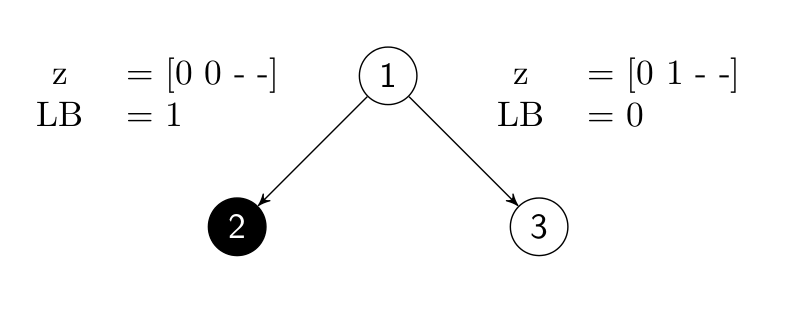
\includegraphics[width=0.45\textwidth]{tree1}
\caption{Tree illustrating the known variables for the nodes and the lower bounds determined by the
variables. A white node represents a branch which should be explored, while a black node represents a
branch which should be pruned.}
\label{fig:tree1}
\end{figure}

Figure~\ref{fig:tree1} shows the root created with $x_1$ = 0, and then the branching of $y_1$. The calculation
of the lower bound for the two child nodes is the done is parallel. Additionally the computation is done in
parallel as explained in Section~\ref{sec:bounding}. Two threads are used, one for the top summation over $j$,
and another for the bottom summation over $j$. Thus for $i$ = 1, the first thread uses $j$ = $J_{1,0}$ = 1 and
computes
\begin{align*}
    \textrm{partial sum} &= c_1(1 - x_1 - y_1 + 2t_{1,1} \\
                         &= 1(1 - 0 - 0) = 1
\end{align*}
simultaneously, the other thread uses $j$ = $J_{1,1}$ = 2 and computes
\begin{align*}
    \textrm{partial sum} &= c_1(y_1 + x_2 + 2t_{1,2} \\
                         &= 1(1 - 0 - 0) = 1
\end{align*}
but since $x_2$ is not know, it does not return a value. The lower bound is then 1, since only the result of
the first thread is used.

\begin{figure}[t!]
    \centering
    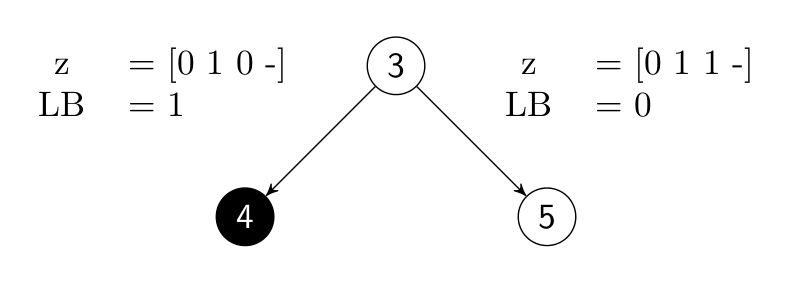
\includegraphics[width=0.45\textwidth]{tree3}
    \caption{Tree illustrating the known variables for the nodes and the lower bounds determined by the
    variables. A white node represents a branch which should be explored, while a black node represents a
branch which should be pruned.}
    \label{fig:tree3}
\end{figure}
\begin{figure}[b!]
    \centering
    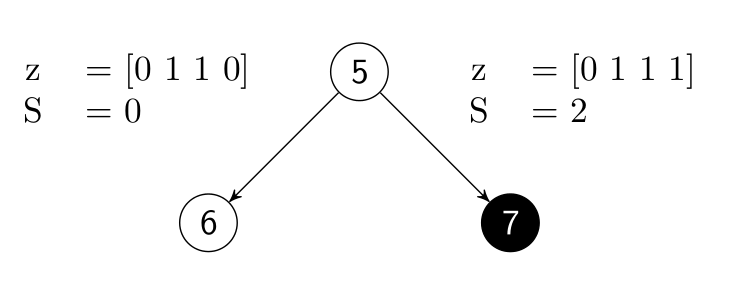
\includegraphics[width=0.45\textwidth]{tree5}
    \caption{Tree illustrating the known variables for the nodes and the scores of each of the branches.}
    \label{fig:tree5}
\end{figure}

At the same time, the lower bound of the right branch would have been computed using the same procedure to
determine the lower bound of 0 as shown in Figure~\ref{fig:tree1}.
Since the lower bound of the left branch is higher than that of the right branch, the branch is pruned and
will not be explored further. Node 3, however, must be explored so 2 new threads are created for branching, 
and the same procedure is applied in parallel. The known variables and the resulting lower bounds for
this are shown in Figure~\ref{fig:tree3}

Node 4 in Figure~\ref{fig:tree3} has a lower bound of 1, which is higher than the lower bound of node 5, which
is 0. Node 4 is pruned while new threads are created to explore node 5 further. Since there is only one
variable left for branching, the two child nodes from node 5 return the score of the branch rather than the lower
bound since the child nodes are leaves. Figure~\ref{fig:tree5} shows the results of branchinf from node 5,
annd the scores of the branch.

Since the leaves of the branch have been found, the lowest score (in this case the score of node 6) is return
to the root of the tree, where is is compared to the solutions of all the other branches to determine which
solution is optimal. In this case, the solution would be $x_1$ = 0, $x_2$ = 1, $y_1$ = 1, $y_2$ = 0, which is
the optimal solution for all branches for this example. Since the concatination of the $x$ variables is the 
solution for the haplotype $h$, $h_{3,4}$ = [$x_1$, $x_2$] = [0,1] which can be verified by
Table~\ref{tab:exinp}.

\begin{thebibliography}{99}
    \bibitem{chenapp:2013}
        Z.-Z. Chen, F. Deng, and L. Wang. Exact al-
        gorithms for haplotype assembly from whole-
        genome sequence data. 29(16):1938–1945, 2013.
\end{thebibliography}

\end{document}

